\documentclass[]{article}
\usepackage{graphicx}

\begin{document}
\begin{titlepage}
\begin{center}
	\includegraphics[scale=0.25]{/home/dieguito/Pictures/logo_udeg_negro.png}\\
	\vspace{1cm}
{\Large 	\textbf{Centro Universitario de Ciencias Exactas e Ingenierías}\\}

\vspace{0.5cm}
	
{\large 	\textit{Departamento de ciencias computacionales}\\}
	
	\vspace{1cm}
	
	\textbf{Administración de redes}\\
	
	\vspace{0.5cm}
	
	\textbf{Reporte semanal}\\
	
	\vspace{0.5cm}
	
	Semana \textbf{3}
	
	\vspace{0.5cm}
	
	\underline{Creación de cables UTP}\\
	
	\vspace{1cm}
	
	Prof: Ing. Luis Ignacio Sánchez Salazar\\
	
	Alumno: Diego Martín Domínguez Hernández\\
	
	Carrera: Ingeniería Informática \\
	
	Materia: i5907 (Administración de Redes)\\
	
	NRC: 42241\\
	
	Sección: D04\\

	Calendario: 2023A\\
	
\end{center}
\end{titlepage}
De las actividades principales en la semana 3, se vio la creación
de un cable UTP, las especificaciones de los cables de conexión de
redes y cómo conectar un cuarto.

El cable UTP es una de las variedades más utilizadas en el ámbito de las conexiones a internet, por la gran cantidad de información que pueden transmitir, la precisión con la que realizan estos trabajos y la rapidez, que son aspectos muy importantes para el cumplimiento del cometido por el que se recurre a estos sistemas.

Así, el cable UTP es una solución muy presente en este sector, especialmente en las conexiones de redes LAN o de área local, aunque también puede verse en otras modalidades de redes.

Su nombre se debe a las siglas en inglés de Unshielded Twisted Pair, lo que en castellano se traduce como par trenzado no apantallado, para diferenciarse de las otras dos alternativas.

Para entender cómo son los cables UTP y la importancia que tienen en el trabajo de los expertos de este sector, es conveniente tener claro que no tienen una protección adicional, a excepción de una cubierta elaborada a base de PVC, pero sin situar ninguna separación entre cada par de su interior.

A causa de su composición, la impedancia que puede ofrecer es de unos 100 Ohm, que es la más inferior respecto a las que pueden soportar los cables STP y cables FTP.

El cable UTP, al igual que el FTP, se vale del conector RJ45, más voluminoso que el utilizado en teléfonos RJ11 pero de similares características.

En realidad, una de las bazas más destacadas del uso del cable UTP es su coste, más asequible que cualquiera de sus alternativas, así como su fácil accesibilidad y la sencillez con la que se puede instalar.

Por ello, se trata de una de las alternativas más extendidas para crear sistemas de conexión eficientes y seguros.

No obstante, al no disponer de la protección en forma de pantalla, son más frágiles y propensos a ver mermada su capacidad por posibles interferencias o la acción de distintos agentes externos.\\


\includegraphics[scale=0.5]{identifying a calbe}

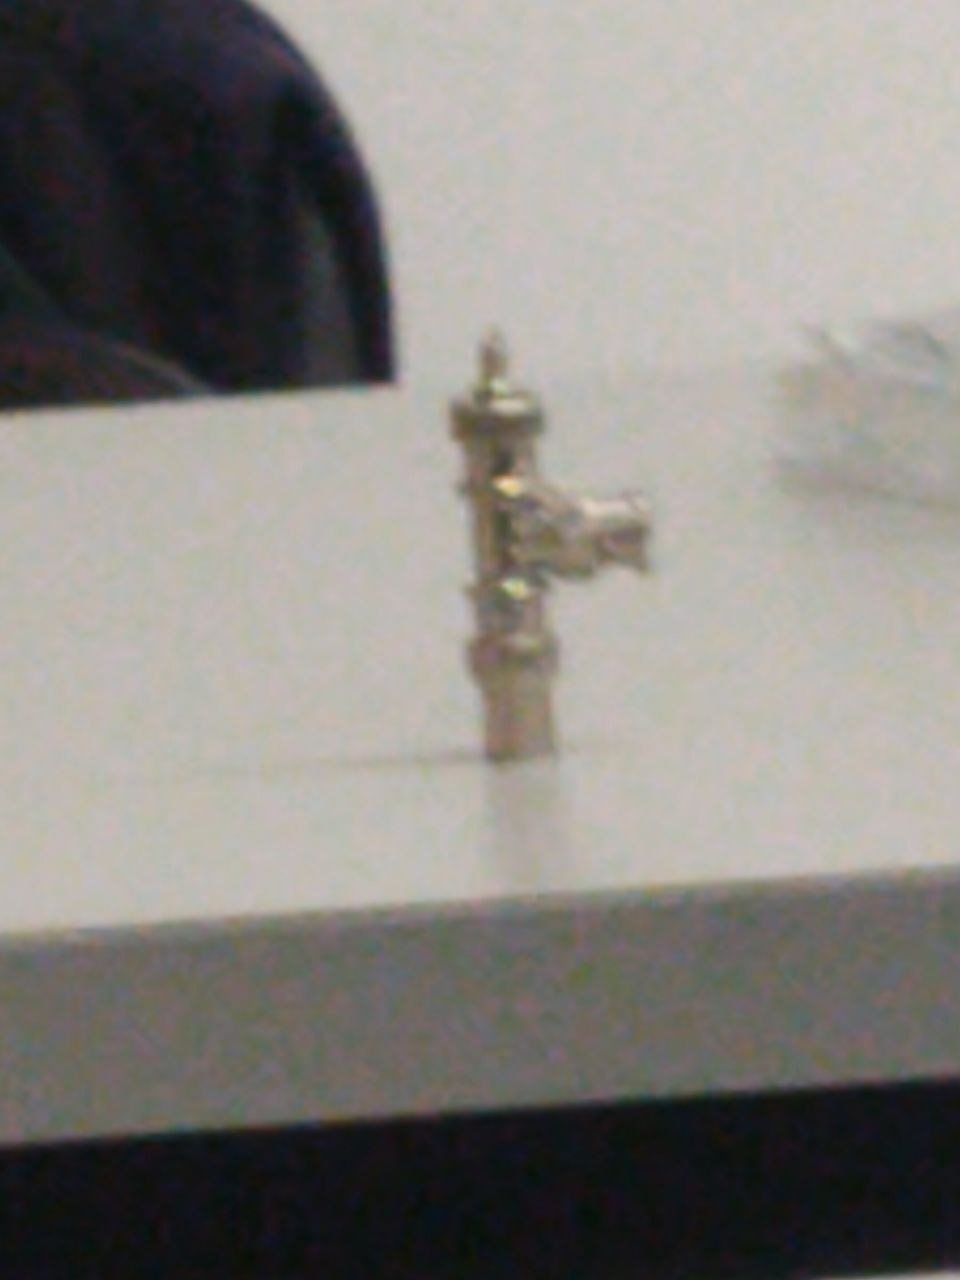
\includegraphics[scale=0.25]{a}

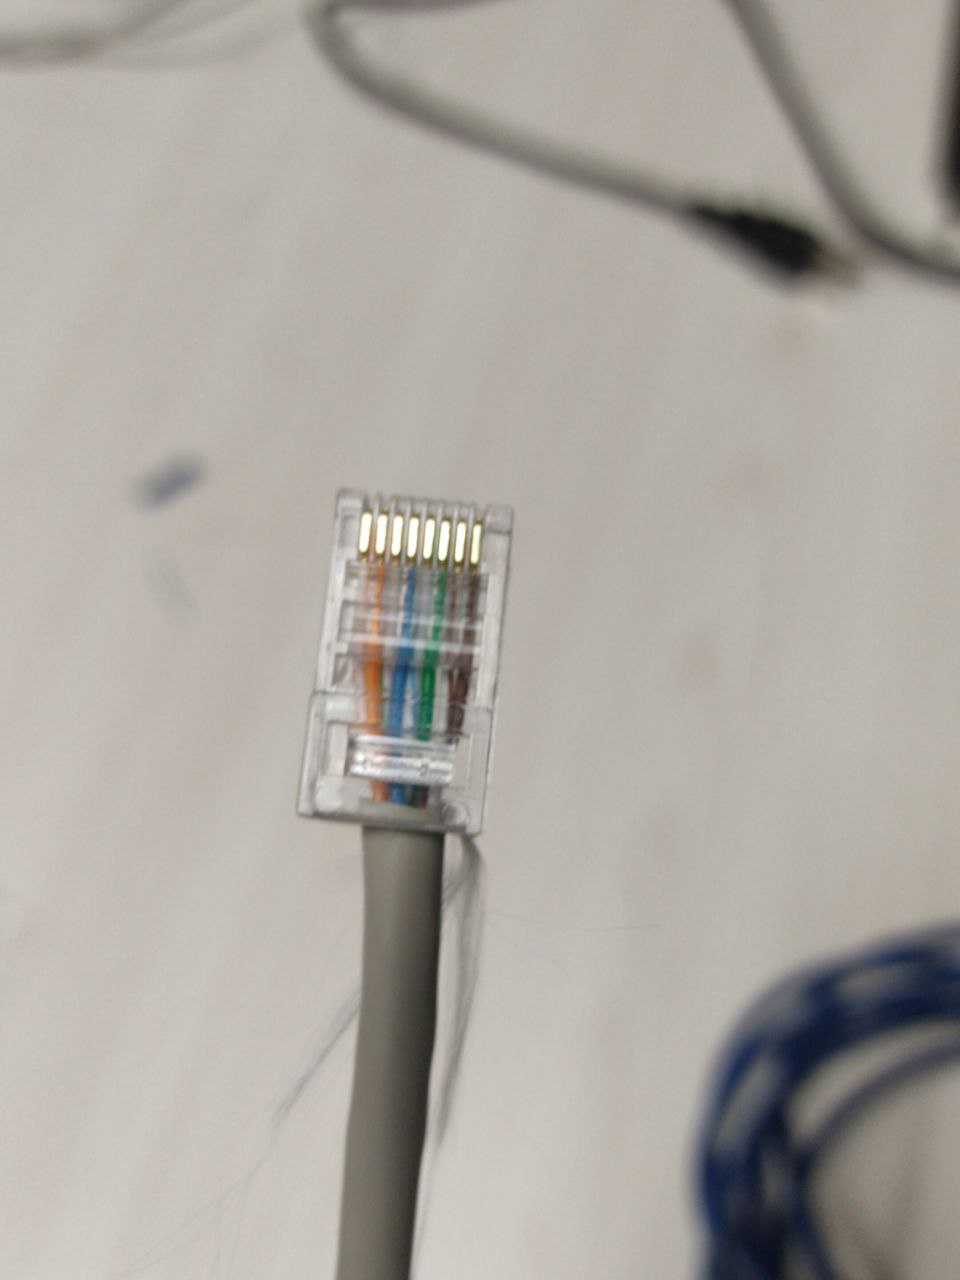
\includegraphics[scale=0.25]{b}

\end{document}